% =========================================================================
% LaTeX document using the IEEEtran class for a conference paper
% =========================================================================
\documentclass[conference]{IEEEtran}

% =========================================================================
% REQUIRED PACKAGES
% =========================================================================
\usepackage{cite}          % Handles citations in IEEE style
\usepackage{amsmath,amssymb,amsfonts} % Math packages
\usepackage{graphicx}      % For including images
\usepackage{textcomp}      % Additional text symbols
\usepackage{xcolor}        % For text coloring
\usepackage{url}           % For formatting URLs
\usepackage{ulem}          % For underlining (\uline)

% For hyperlinking URLs and citations
\usepackage{hyperref}
\hypersetup{
    colorlinks=true,
    linkcolor=blue,
    filecolor=magenta,
    urlcolor=blue,
    citecolor=black, % IEEE style often has black citation numbers in text
}

% Ensure that figures are placed reasonably
\usepackage{float}

% Correct bad hyphenation here
\hyphenation{op-tical net-works semi-conduc-tor}


% =========================================================================
% BEGIN DOCUMENT
% =========================================================================
\begin{document}

% =========================================================================
% TITLE AND AUTHOR INFORMATION
% =========================================================================
\title{On-Device Personalized Agent using Fine-tuned Qwen3-0.6B}

\author{\IEEEauthorblockN{Brandon Howell}
\IEEEauthorblockA{\textit{Department Name or Project Group} \\
\textit{University or Organization Name}\\
City, Country \\
Email: your.email@example.com}
}

% Make the title area
\maketitle

% =========================================================================
% ABSTRACT AND KEYWORDS
% =========================================================================
\begin{abstract}
This project aims to create a personalized AI assistant capable of running directly on an Android smartphone. The core of this work involves fine-tuning a small large language model (LLM), specifically Qwen3-0.6B, with personal user data to create a private, context-aware agent. This personalized model is then integrated into an experimental Android agent framework, based on Gosling, to enable it to perform tasks by interacting with other applications on the device. We address the significant challenges of on-device LLM inference, user data privacy, and agentic control within the resource-constrained and complex mobile environment. The project explores the trade-offs between full fine-tuning and parameter-efficient fine-tuning (PEFT) techniques to achieve a capable yet efficient personalized agent.
\end{abstract}

\begin{IEEEkeywords}
On-Device AI, Small Language Models, LLM Personalization, Agentic AI, Parameter-Efficient Fine-Tuning (PEFT), Android, Qwen3.
\end{IEEEkeywords}


% =========================================================================
% SECTIONS
% =========================================================================

\section{Introduction}

\textit{\uline{Scope:}} This project aims to create a personalized AI assistant capable of running directly on an Android smartphone. The core involves fine-tuning a small, large language model (LLM), specifically Qwen3-0.6B~\cite{qwen}, with personal user data and other Android domain specific information. Subsequently, this personalized model will be integrated into an experimental Android agent framework (potentially a fork of Gosling~\cite{gosling}) to enable it to perform tasks by interacting with other applications on the device.

\textit{\uline{Problem:}} Current large language models, while powerful, are typically generic and operate in the cloud, which raises privacy concerns and lacks deep personalization. Running large models locally on resource-constrained devices like smartphones is computationally challenging. Enabling these models to interact with the device's applications and data in an automated fashion (i.e., act as agents) presents significant technical hurdles in the mobile environment. This project addresses the need for a private, personalized, and capable AI assistant that lives entirely on a user's device.

\textit{\uline{Interest \& Non-Triviality:}} This project is interesting because it tackles the intersection of several cutting-edge AI domains:
\begin{itemize}
    \item \textit{\uline{On-Device AI:}} Deploying capable LLMs on mobile phones pushes the boundaries of model optimization and efficient inference while preserving privacy.
    \item \textit{\uline{LLM Personalization:}} Fine-tuning with personal data explores methods to make AI truly tailored to an individual user's context, habits, and preferences.
    \item \textit{\uline{Agentic AI on Mobile:}} Integrating an LLM with device automation frameworks like Gosling explores the practical challenges and potential of creating autonomous agents in the complex and varied Android ecosystem.
    \item \textit{\uline{Parameter-Efficient Fine-Tuning (PEFT):}} Experimenting with techniques like adapters offers insights into efficient model adaptation for resource-constrained environments.
\end{itemize}

The combination of fine-tuning a recent small LLM, deploying it locally, integrating personal context, and building agentic capabilities makes this project ambitious and non-trivial. A conceptual diagram is shown in Fig.~\ref{fig:mobile_agent}.

\begin{figure}[t]
\centering
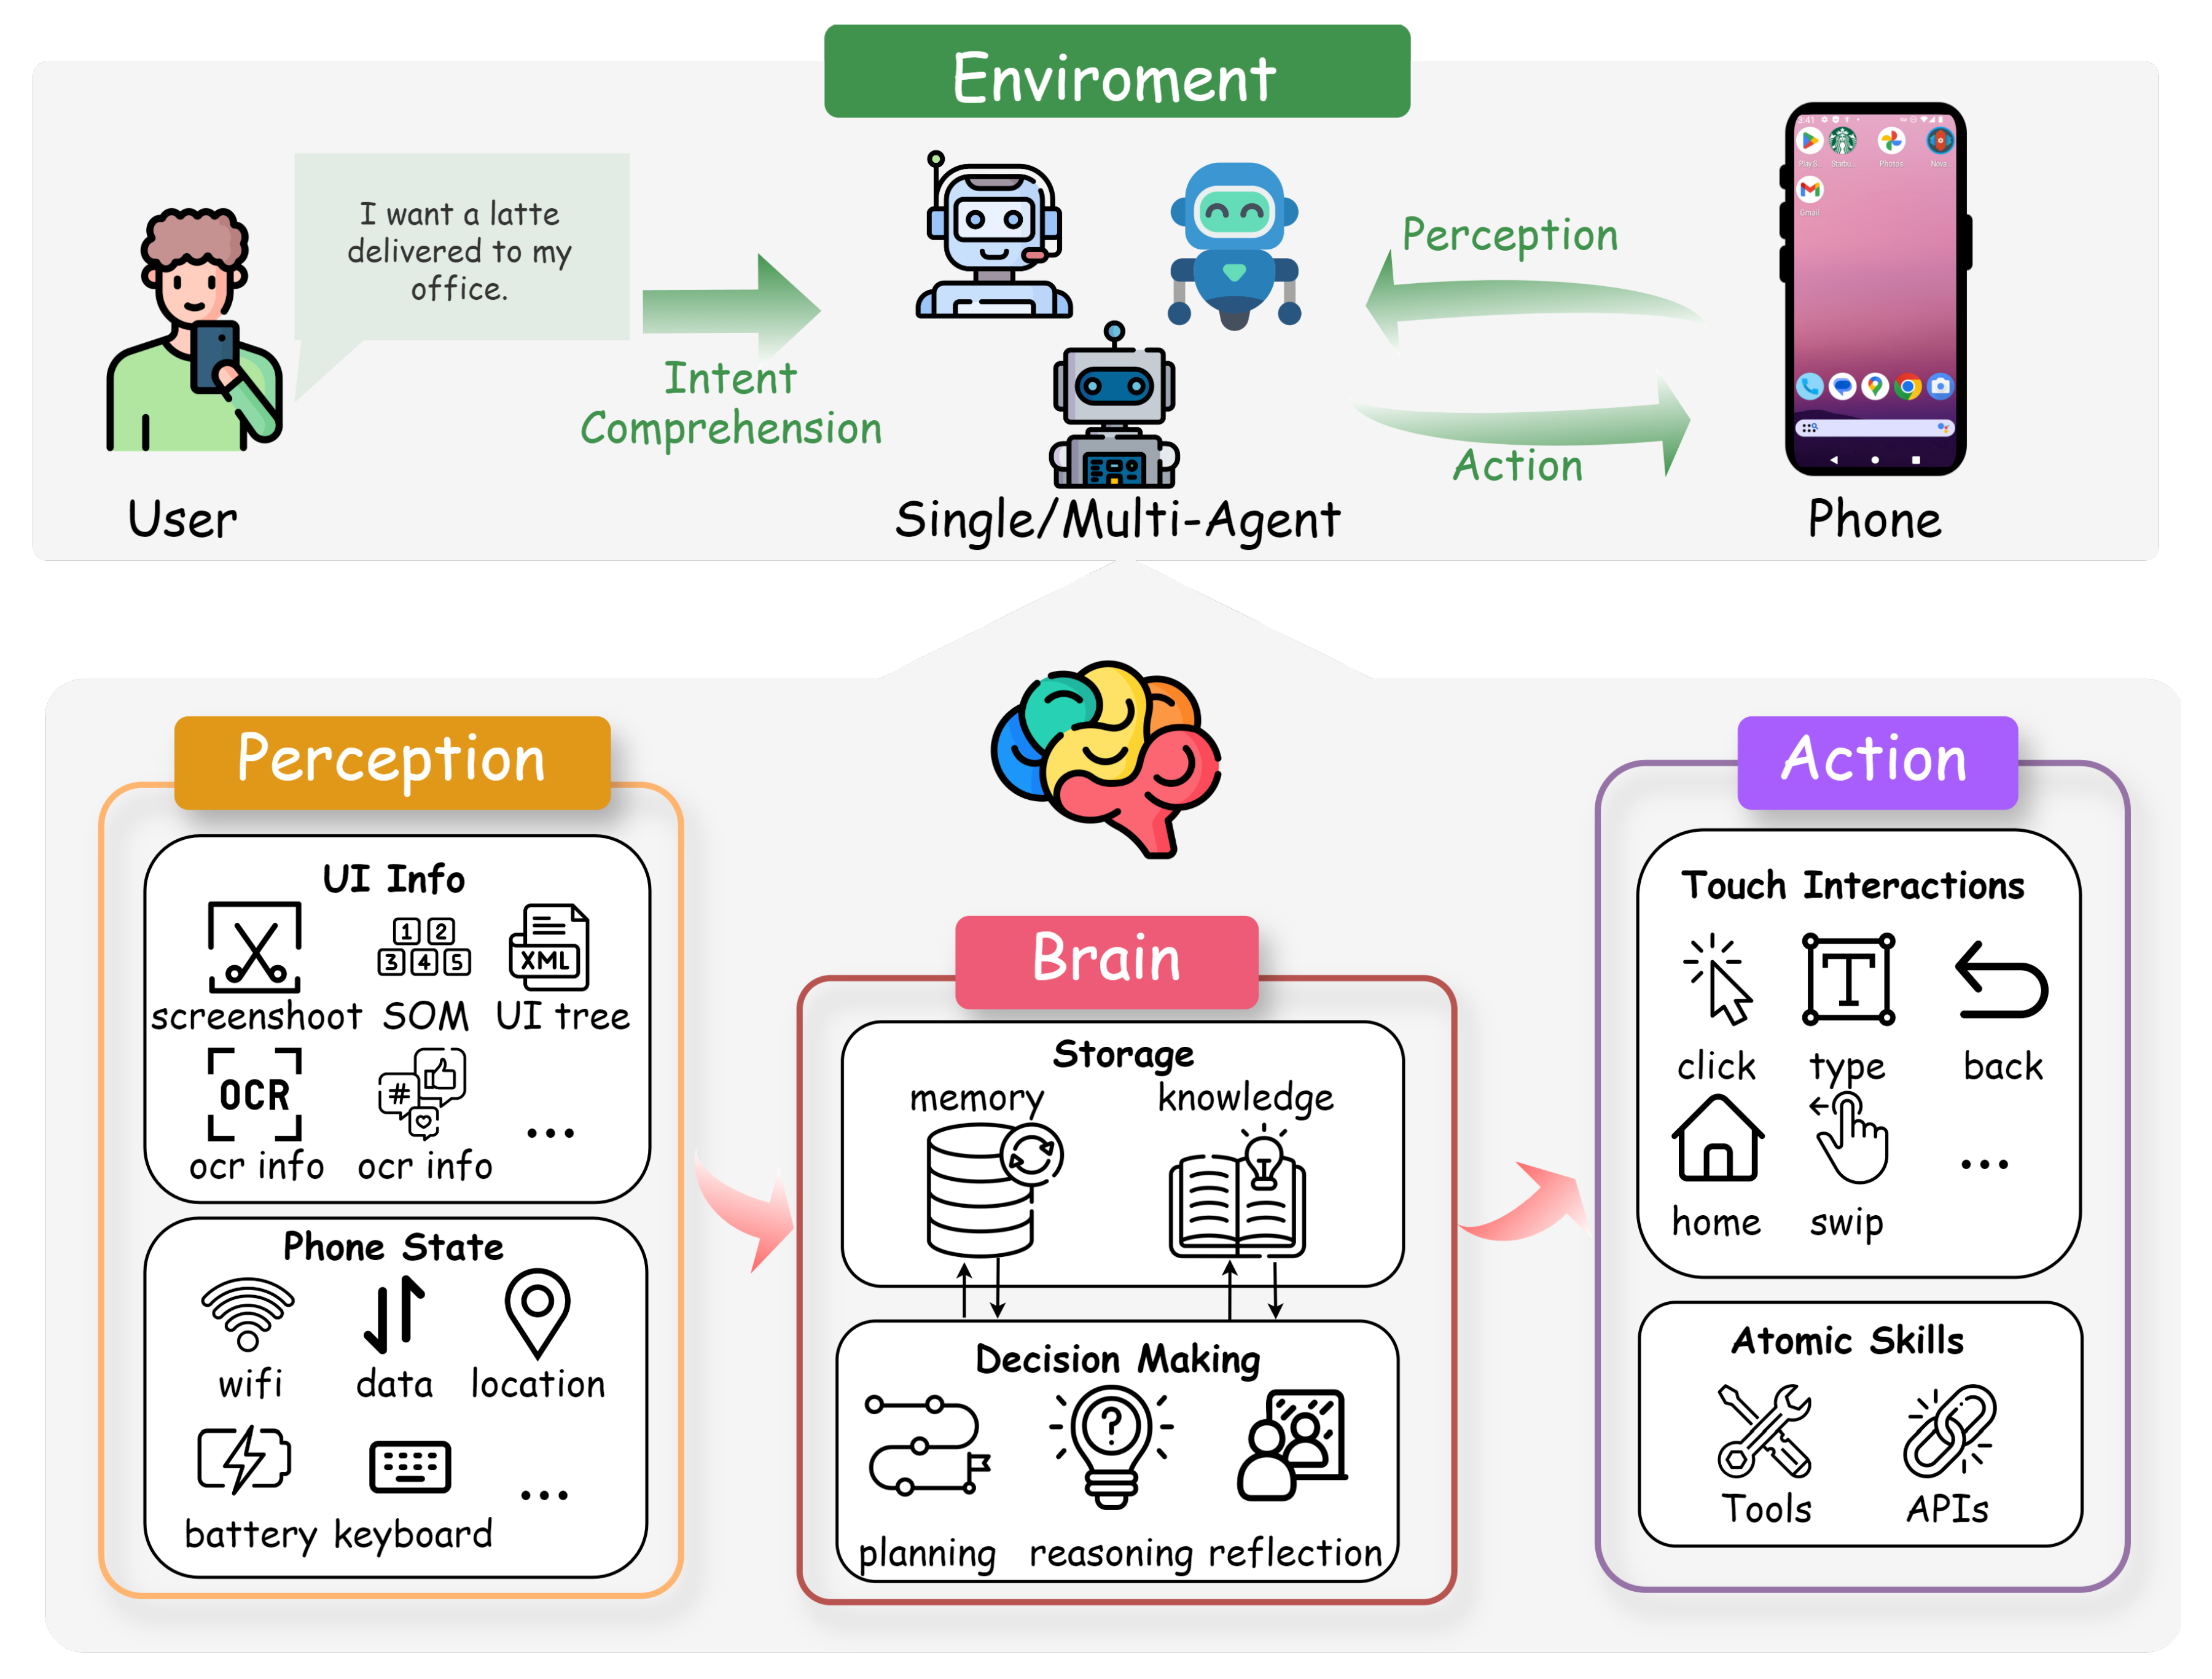
\includegraphics[width=0.9\linewidth]{images/mobile_agent_image.png}
\caption{Conceptual diagram of a mobile LLM agent architecture, where the agent reasons about user tasks and interacts with applications on the device. Image from~\cite{mobileagentimage}.}
\label{fig:mobile_agent}
\end{figure}

\section{Related Work}
The development of personalized, on-device AI agents draws upon research in several areas.

\textit{\uline{Small Language Models (SLMs):}} The trend towards smaller, capable language models is necessary for on-device deployment. Models like Phi-3, Gemma, and the chosen Qwen3-0.6B~\cite{qwen} from Alibaba represent efforts to achieve high performance with fewer parameters. The Qwen3 series specifically notes optimization for resource-constrained environments~\cite{qwen3blog}.

\textit{\uline{On-Device LLM Inference:}} Techniques for efficiently running LLMs on mobile devices are critical. This includes model quantization, optimized inference engines (like \texttt{llama.cpp}, MediaPipe LLM Inference, ONNX Runtime), and leveraging mobile NPUs/GPUs~\cite{efficiency}.

\textit{\uline{LLM Fine-Tuning for Personalization:}} Adapting pre-trained LLMs is a common practice. While full fine-tuning is resource-intensive, \textbf{Parameter-Efficient Fine-Tuning (PEFT)} methods have gained prominence. Techniques like Adapter Tuning~\cite{adapterspaper}, LoRA~\cite{lora}, and QLoRA~\cite{qlora} allow adaptation by training only a small number of additional parameters, as illustrated in Fig.~\ref{fig:adapters}. This is particularly relevant for on-device scenarios.

\begin{figure}[t]
\centering
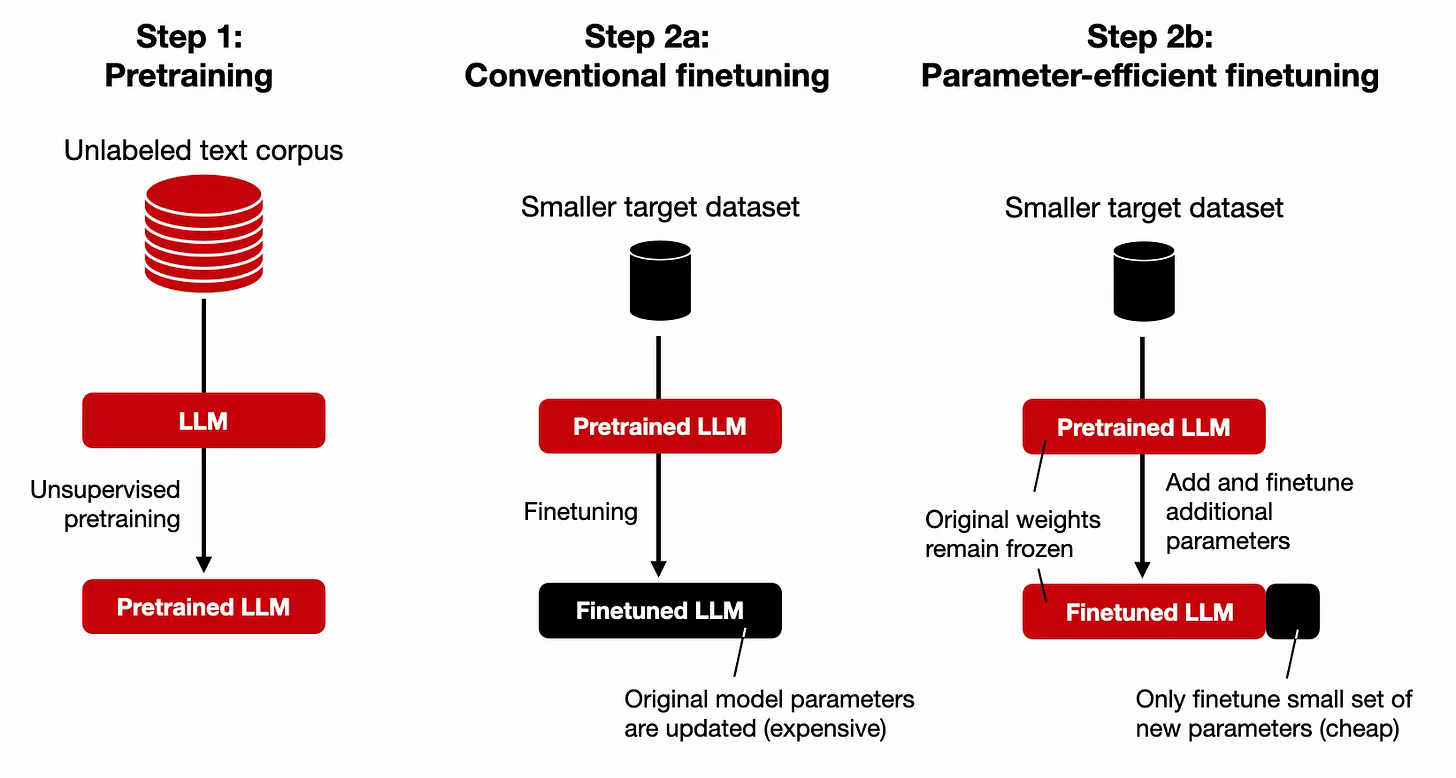
\includegraphics[width=0.9\linewidth]{images/adapters.png}
\caption{Illustration of adapter-based PEFT. Small, trainable adapter modules are inserted into a frozen pre-trained model, enabling efficient fine-tuning. Image from~\cite{adaptersimage}.}
\label{fig:adapters}
\end{figure}

\textit{\uline{LLM-Powered Agents:}} Frameworks enabling LLMs to use tools and execute tasks are emerging. Applying these concepts to mobile environments involves interacting with apps and system services. Projects like Gosling~\cite{gosling} specifically explore agentic capabilities on Android, using platform features like Accessibility Services.

\section{Method}
This project is developed in two main phases.

\subsection{Phase 1: Personalized On-Device LLM Fine-tuning}
\begin{enumerate}
    \item \textit{\uline{Model Selection:}} The core model is Qwen3-0.6B, chosen for its small size and performance~\cite{qwen}.
    \item \textit{\uline{Data Collection \& Preparation:}} A personal dataset will be curated, including calendar entries, synthesized communication logs, personal notes, app usage patterns, and location habits. The data will be formatted for instruction fine-tuning.
    \item \textit{\uline{Fine-tuning Implementation:}} Two approaches will be explored using Hugging Face \texttt{transformers} and \texttt{peft}:
    \begin{itemize}
        \item \textbf{Full Fine-tuning:} Update all weights of the model.
        \item \textbf{Adapter-based PEFT:} Freeze the base model and train lightweight adapter modules~\cite{adapterspaper, lora, qlora}.
    \end{itemize}
    \item \textit{\uline{On-Device Deployment:}} The fine-tuned models will be prepared for on-device execution via quantization (e.g., 4-bit GGUF) and deployed using an inference engine like \texttt{llama.cpp} with Android bindings.
\end{enumerate}

\subsection{Phase 2: Agentic Integration with Gosling}
\begin{enumerate}
    \item \textit{\uline{Framework Setup:}} Fork the Gosling Android agent repository and study its architecture for invoking LLMs and interacting with device capabilities.
    \item \textit{\uline{Model Integration:}} Modify the forked Gosling code to use the personalized, locally deployed Qwen3-0.6B model (likely the PEFT version) as its reasoning engine.
    \item \textit{\uline{Tool Definition \& Use:}} Explore Gosling's mechanisms for defining and using tools, potentially implementing custom capabilities via a "mobile MCP" provider.
    \item \textit{\uline{Task Automation:}} Define and test simple, multi-step tasks that require the agent to use the personalized LLM and interact with other apps via Gosling's capabilities.
\end{enumerate}

\section{Evaluation}
Success will be evaluated based on experimentation depth and insights gained.

\subsection{Phase 1 Evaluation (Personalized LLM)}
\begin{itemize}
    \item \textit{\uline{Dataset:}} A held-out set of prompts based on the personal data domain.
    \item \textit{\uline{Metrics:}}
    \begin{itemize}
        \item \textbf{Qualitative Assessment:} Subjective evaluation of the model's responses for personalization, accuracy, coherence, and tone compared to the base model.
        \item \textbf{Quantitative Assessment (Exploratory):} Measure perplexity, model storage size, inference latency, and peak memory usage on the Android device.
    \end{itemize}
    \item \textit{\uline{Comparison:}} Directly compare the effectiveness and resource trade-offs between the fully fine-tuned and adapter-based models.
\end{itemize}

\subsection{Phase 2 Evaluation (Agentic Capabilities)}
\begin{itemize}
    \item \textit{\uline{Dataset:}} A set of defined, multi-step tasks requiring interaction with device features or apps.
    \item \textit{\uline{Metrics:}}
    \begin{itemize}
        \item \textbf{Task Completion Rate:} Percentage of tasks successfully completed.
        \item \textbf{Qualitative Assessment:} Evaluate planning ability, tool usage effectiveness, error handling, and overall usefulness.
        \item \textbf{Efficiency (Observational):} Note the time and steps required for task completion.
    \end{itemize}
\end{itemize}

\section{Milestones}
The project timeline is structured as follows:
\begin{itemize}
    \item \textit{\uline{Week 6:}} Download Qwen model, test baseline capabilities, and begin curating the fine-tuning dataset.
    \item \textit{\uline{Week 7:}} Fine-tune and test the personalized model. Evaluate its qualitative and quantitative improvements over the base model.
    \item \textit{\uline{Week 8:}} Fork the Gosling repository and begin integration work for the agent framework.
    \item \textit{\uline{Week 9:}} Combine the fine-tuned Qwen3 with Gosling to automate tasks. Test and gather quantitative results on task success.
    \item \textit{\uline{Week 10:}} Finalize features, complete testing and evaluations, and prepare the final report.
\end{itemize}

\section{Task Assignments}
This is a solo project, so all tasks will be handled by the author.

% =========================================================================
% BIBLIOGRAPHY
% =========================================================================

\bibliographystyle{IEEEtran}
\bibliography{references}

% =========================================================================
% END DOCUMENT
% =========================================================================
\end{document}
